\documentclass[12pt,a4paper]{report}
\usepackage[utf8]{inputenc}
\usepackage{geometry}
\geometry{margin=1in}
\usepackage{graphicx}
\usepackage{setspace}
\usepackage{titlesec}
\usepackage{tocloft}
\usepackage{hyperref}
\usepackage{tabularx}
\usepackage{float}
\usepackage{enumitem}
\usepackage{xcolor}
\definecolor{maroon}{RGB}{128,0,0}

\begin{document}
\setstretch{1.5}

% -------------------------
% TITLE PAGE
% -------------------------
\begin{titlepage}
    \centering
    \vspace*{1cm}
    
    {\Huge \textbf{Roommate Finder Platform} \par}
    
    \vspace{1.5cm}
    
    {\Large Summer Internship Project Report for \par}
    {\Large DataValley - APSCHE \par}
    
    \vspace{1.5cm}
    
    {\Large \textbf{Submitted by:} \par}
    \vspace{0.5cm}
    {\large N210390 - I. Uma Manikanta \par}
    
    \vspace{1.5cm}
    
    {\Large \textbf{Under the Esteem Guidance of} \par}
    {\large Mrs. M. Jyothi \par}
    {\large Asst. Professor, Department of CSE \par}
    
    \vspace{2cm}
    

    
    {\LARGE \textbf{RGUKT} \par}
    \vspace{1cm}
    
    {\large \textbf{Department of Computer Science and Engineering} \par}
    {\large Rajiv Gandhi University of Knowledge Technologies, Nuzvid \par}
    
    \vspace{0.5cm}
    {\large Internship Period: 6th of May, 2026 to 28th of June 2026 \par}
\end{titlepage}

\newpage
\thispagestyle{empty}
\mbox{}
\newpage

\pagenumbering{roman}

% -------------------------
% CERTIFICATE OF COMPLETION
% -------------------------
\chapter*{\centering \Large \textcolor{maroon}{CERTIFICATE OF COMPLETION}}
\addcontentsline{toc}{chapter}{CERTIFICATE OF COMPLETION}
\vspace{1cm}
This is to certify that the work entitled, \textbf{``ROOMMATE FINDER PLATFORM''} is the Bonafide work of \textbf{IKKURTHI UMA MANIKANTA} with ID No: \textbf{N210390} carried out under my guidance and supervision as a Summer Internship Project at \textbf{DataValley} - APSCHE. This work is done during the period \textbf{6th of May, 2026 to 28th of June 2026}, under our guidance.

\vspace{3cm}
\noindent
\begin{minipage}{0.5\textwidth}
\textbf{Mrs. M. Jyothi} \\
Assistant Professor, \\
Department of CSE, \\
RGUKT-Nuzvid
\end{minipage}%
\hfill
\begin{minipage}{0.45\textwidth}
\begin{flushright}
\textbf{Mr. A. Uday Kumar} \\
Head of Department, \\
Department of CSE, \\
RGUKT - Nuzvid
\end{flushright}
\end{minipage}
\newpage

% -------------------------
% CERTIFICATE OF EXAMINATION
% -------------------------
\chapter*{\centering \Large \textcolor{maroon}{CERTIFICATE OF EXAMINATION}}
\addcontentsline{toc}{chapter}{CERTIFICATE OF EXAMINATION}
\vspace{1cm}
This is to certify that the work entitled, \textbf{``ROOMMATE FINDER PLATFORM''} is the Bonafide work of \textbf{IKKURTHI UMA MANIKANTA} with ID No: \textbf{N210390} and hereby accord our approval of it as a study carried out during the summer internship at \textbf{DataValley} - APSCHE, and presented in a manner required for its acceptance. This approval does not necessarily endorse or accept every statement made, opinion expressed or conclusion drawn, as recorded in this thesis. It only signifies the acceptance of this thesis for the purpose for which it has been submitted.

\vspace{3cm}
\noindent
\begin{minipage}{0.5\textwidth}
\textbf{Mrs. M. Jyothi} \\
Assistant Professor, \\
Department of CSE, \\
RGUKT-Nuzvid
\end{minipage}%
\hfill
\begin{minipage}{0.45\textwidth}
\begin{flushright}
\textbf{Project Examiner} \\
1. Mr. G. Jaya Krishna \\
2. Mrs. B. Padma Bai \\
Assistant Professor, \\
Department of CSE, \\
RGUKT-Nuzvid
\end{flushright}
\end{minipage}
\newpage

% -------------------------
% DECLARATION
% -------------------------
\chapter*{\centering \Large \textcolor{maroon}{DECLARATION}}
\addcontentsline{toc}{chapter}{DECLARATION}
\vspace{1cm}
I, \textbf{IKKURTHI UMA MANIKANTA} with ID No: \textbf{N210390} hereby declare that the project report entitled \textbf{``ROOMMATE FINDER PLATFORM''} done by me under the guidance of \textbf{Mrs. M. Jyothi} is submitted for the partial fulfillment of the Summer Internship at \textbf{DataValley} - APSCHE during the period \textbf{6th of May, 2026 to 28th of June 2026}.

I also declare that this project is a result of my own effort and has not been copied or imitated from any source. Citations from any websites are mentioned in the references. The results embodied in this project report have not been submitted to any other university or institute for the award of any degree or diploma.

\vspace{2cm}
\noindent Date : \hrulefill \\
\vspace{1cm} \\
\noindent Place : \hrulefill
\newpage

% -------------------------
% ACKNOWLEDGEMENT
% -------------------------
\chapter*{\centering \Large \textcolor{maroon}{ACKNOWLEDGEMENT}}
\addcontentsline{toc}{chapter}{ACKNOWLEDGEMENT}
\vspace{1cm}
I would like to express my profound gratitude and deep regards to my guide \textbf{Mrs. M. Jyothi} for her exemplary guidance, monitoring, and constant encouragement. I shall always cherish the time spent with her during the course of this work due to the invaluable knowledge gained in the field of software engineering and full-stack web development.

I am extremely grateful to the team at \textbf{DataValley} for the confidence bestowed upon me and for entrusting me with the project entitled \textbf{``Roommate Finder Platform''} during my summer internship.

I express my gratitude to \textbf{Mr. A. Uday Kumar} (HOD of CSE) and other faculty members for being a source of inspiration and constant encouragement, which helped me in completing the project successfully.

I am also thankful to our Director, \textbf{Prof. SSSV Gopala Raju} for giving me the opportunity to do this project.
\newpage

% -------------------------
% TABLE OF CONTENTS & LISTS
% -------------------------
\tableofcontents
\newpage

\listoffigures
\addcontentsline{toc}{chapter}{LIST OF FIGURES}
\newpage

\listoftables
\addcontentsline{toc}{chapter}{LIST OF TABLES}
\newpage

% -------------------------
% ABSTRACT
% -------------------------
\chapter*{Abstract}
\addcontentsline{toc}{chapter}{Abstract}
Finding a compatible roommate and suitable living arrangement is a pervasive challenge for students and young professionals relocating to new cities or entering higher education. Traditional methods of finding roommates typically involve browsing unstructured social media groups, unverified forum listings, or word-of-mouth recommendations. These manual processes are time-consuming, inherently risky regarding personal security, and highly prone to resulting in mismatched living styles, which can lead to uncomfortable living situations and premature lease terminations. 

This project proposes an automated, intelligent \textbf{Roommate Finder Platform} designed to bridge this gap by providing a secure, user-friendly, and data-driven approach to roommate pairing. The system transitions the roommate search process from a manual, property-centric model to an automated, user-centric matchmaking experience. 

The platform is developed using a modern full-stack web architecture, specifically the MERN (MongoDB, Express.js, React.js, Node.js) stack. It incorporates secure user authentication mechanisms utilizing JSON Web Tokens (JWT) and bcrypt password hashing. Furthermore, it features a robust user profiling system that captures essential lifestyle habits, budget constraints, and personal preferences. At the core of the platform is a customized matching algorithm that computes compatibility scores between users by dynamically weighting overlapping preferences and filtering out absolute deal-breakers.

The proposed platform was developed and rigorously tested to handle real-world scenarios. Experimental evaluations of the API endpoints indicate low latency and high throughput, while functional testing validates the accuracy of the matching algorithm. The resulting application significantly reduces the time and effort required to find a highly compatible roommate, thereby enhancing user safety and fostering more harmonious living environments.

\newpage
\pagenumbering{arabic}

% -------------------------
% CHAPTER 1: INTRODUCTION
% -------------------------
\chapter{INTRODUCTION}

\section{Overview}
Urbanization and the centralization of higher education have led to a massive influx of young adults migrating to metropolitan areas and college towns. One of the most immediate and stressful challenges these individuals face upon relocation is securing affordable housing. Due to the high cost of living, sharing an apartment or housing unit with roommates has become an economic necessity rather than a mere choice. However, the process of finding a roommate is fraught with difficulties, as living with a stranger requires a high degree of trust and lifestyle compatibility. 

Communication and mutual respect are fundamental to a harmonious living arrangement. When individuals rely on unstructured platforms to find housing partners, they often lack the tools to assess compatibility before committing to a lease. This project, the Roommate Finder Platform, introduces a structured, technology-driven solution to mitigate these challenges.

\section{Motivation for the Work}
The motivation for this project stems from the critical limitations and systemic flaws present in existing housing and roommate search methods:
\begin{itemize}
    \item \textbf{Inadequacy of Unstructured Platforms:} Traditional search methods utilize generic classifieds (e.g., Craigslist) or social media groups (e.g., Facebook Housing Groups). These platforms lack structured data schemas. Users post paragraphs of text that cannot be filtered or sorted algorithmically, failing to systematically capture critical compatibility metrics such as sleep schedules, cleanliness habits, dietary restrictions, and social inclinations.
    \item \textbf{Security and Verification Concerns:} Early attempts at finding roommates often involve interacting with entirely unverified strangers. These interactions are inherently risky and highly prone to fraudulent activities, such as housing scams or identity theft. There is a pressing need for a system with robust user authentication and verification protocols.
    \item \textbf{Absence of Compatibility Algorithms:} While basic listing sites excel at showing available rooms based on geographic location and price, they do not match people based on behavioral compatibility. This project explores the implementation of customized matching algorithms as a more efficient alternative to manual filtering. By processing user preferences into quantifiable scores, the system offers matches that have a higher probability of long-term success.
\end{itemize}

\section{Problem Statement}
Current methods for finding roommates are highly decentralized, manual, and lack structural verification. Users are forced to rely on trial-and-error communication across multiple disparate platforms. There is a distinct lack of a centralized web application that not only verifies user identities but also mathematically calculates lifestyle compatibility to recommend the best possible living companions.

\section{Objectives of the Project}
The primary objectives of the Roommate Finder Platform are:
\begin{enumerate}
    \item To design and develop a secure, responsive, and intuitive web-based interface for users to create and manage their housing profiles.
    \item To implement a secure backend infrastructure capable of handling user authentication, session management, and data persistence.
    \item To design a flexible database schema capable of storing diverse user preferences and lifestyle habits.
    \item To engineer a matching algorithm that accurately calculates a compatibility score between users based on shared preferences and weighted lifestyle factors.
    \item To provide a secure platform for matched users to discover and evaluate one another before initiating direct communication.
\end{enumerate}

\section{Scope of the Project}
The scope of this project is confined to the development of the web application and its core algorithmic matching capabilities. The platform targets university students and young working professionals. It encompasses user registration, profile creation (including a comprehensive lifestyle questionnaire), backend matching logic, and a dashboard for viewing potential matches. The scope includes the deployment of a fully functional minimum viable product (MVP) utilizing the MERN stack.

\section{Organization of the Report}
The remainder of this report is organized as follows: Chapter 2 reviews the literature and evolution of existing systems. Chapter 3 details the system architecture, frontend and backend design, and database schema. Chapter 4 provides an in-depth look at the implementation methodology, routing, state management, and the matching algorithm. Chapter 5 discusses the evaluation, performance testing, and UI/UX results. Finally, Chapter 6 concludes the report and outlines potential avenues for future work.

% -------------------------
% CHAPTER 2: LITERATURE REVIEW
% -------------------------
\chapter{LITERATURE REVIEW}

\section{Evolution of Housing and Roommate Search Platforms}
The process of finding a roommate has progressed through several distinct phases of technological evolution. Historically, the search relied entirely on localized, manually designed physical notice boards on college campuses or classified advertisements in local newspapers. While pioneering for their time, these methods struggled with high physical limitations, low visibility, and an inability to convey complex human preferences.

With the advent of the internet (Web 1.0), the search transitioned to digital classifieds. Platforms allowed users to post text-based listings searchable by basic keywords. However, these platforms merely digitized the newspaper experience without adding intelligent processing.

The rise of Web 2.0 introduced database-driven web applications capable of filtering searches based on structured criteria like rent and precise geographic location. Despite this technological leap, the focus remained heavily on the \textit{property} rather than the \textit{people} occupying it.

\section{Unstructured Data vs. Structured Data in Matchmaking}
A significant barrier in roommate matching is the handling of user data. Social media platforms, which currently dominate the informal roommate search market, rely on unstructured data. A user might post, "Looking for a neat roommate who doesn't smoke and goes to bed early." While human-readable, this unstructured text cannot be easily parsed by standard web algorithms to suggest matches.

Modern web applications solve this by employing structured data models (JSON formats) where specific attributes (e.g., `isSmoker: false`, `cleanlinessLevel: 8`) are strictly defined. This structural shift is what enables programmatic matchmaking and sorting.

\section{Algorithmic and Preference-Based Matching Architectures}
Preference-based strategies offer a resilient alternative to simple listing methods by focusing on detailed user profiles, thereby eliminating the noise of incompatible matches programmatically.
\begin{itemize}
    \item \textbf{Profile State Management:} Tools and frameworks like React are now widely used to manage the complex state of a user's multi-step profile creation, ensuring that data is captured seamlessly before being transmitted to the backend.
    \item \textbf{Matching Logic Models:} Backend services now frequently employ scoring algorithms specifically designed to capture compatibility across multiple dimensions. Recent web development trends have explored weighted scoring systems implemented directly in the backend logic, achieving high user satisfaction rates by filtering out incompatible profiles before they reach the client interface.
\end{itemize}

\section{Limitations of Existing Systems}
Despite advancements, many current systems suffer from specific technical and functional limitations:
\begin{itemize}
    \item \textbf{Static Filtering:} Most applications only filter out absolute negatives (e.g., hiding all profiles over a certain budget) but fail to rank the remaining profiles based on nuanced behavioral traits.
    \item \textbf{Poor User Experience (UX):} Legacy platforms often feature outdated, unresponsive user interfaces that do not adapt to mobile devices, frustrating modern users.
    \item \textbf{Security Vulnerabilities:} Many peer-to-peer housing platforms lack proper authentication, making them susceptible to automated bot accounts and phishing schemes.
\end{itemize}

\section{Comparative Summary of Platforms}
The following table summarizes the characteristics and limitations of the primary architectures discussed in the literature compared to our proposed approach:

\begin{table}[H]
\centering
\caption{Comparative Summary of Roommate Search Architectures}
\vspace{0.3cm}
\begin{tabularx}{\textwidth}{|X|X|X|X|}
\hline
\textbf{Architecture / Platform} & \textbf{Primary Focus} & \textbf{Advantages} & \textbf{Primary Limitations} \\
\hline
Classified Ads (e.g., Craigslist) & Location \& Price & High volume of daily listings; easy access. & High scam rate; completely unstructured data; no compatibility check. \\
\hline
Social Media (e.g., Facebook) & Community-based & Easy to communicate; users have existing profiles. & Unstructured data; severe privacy concerns; highly manual search. \\
\hline
Basic Listing Web Apps & Property details \& Amenities & Good UI/UX; verified properties; advanced filtering. & Ignores user lifestyle compatibility; highly property-centric. \\
\hline
\textbf{Proposed System (Our Work)} & \textbf{User Compatibility, Security \& Verification} & \textbf{Algorithmic matching; highly structured preferences; secure JWT backend.} & \textbf{Requires a critical mass of initial users for optimal matching.} \\
\hline
\end{tabularx}
\end{table}

% -------------------------
% CHAPTER 3: SYSTEM ARCHITECTURE AND METHODOLOGY
% -------------------------
\chapter{SYSTEM ARCHITECTURE AND DESIGN}

\section{Proposed Solution Overview}
The proposed solution is an intelligent Roommate Finder platform engineered to provide secure, preference-based matching between individuals. Unlike standard listing systems that focus purely on the physical real estate, this project targets the complex dynamics of human compatibility. 

The system leverages the MERN (MongoDB, Express.js, React.js, Node.js) technology stack to process lifestyle preferences into a quantifiable compatibility score. By utilizing a scalable, decoupled client-server architecture, the solution ensures that users experience a highly responsive interface while complex data routing and matching logic are securely handled on the backend.

\section{High-Level System Architecture}
The system follows a standard 3-Tier Distributed Architecture designed to optimize computational efficiency, maintainability, and user experience. The architecture is divided into the Presentation Layer, Application Layer, and Data Layer.

\begin{figure}[H]
    \centering
    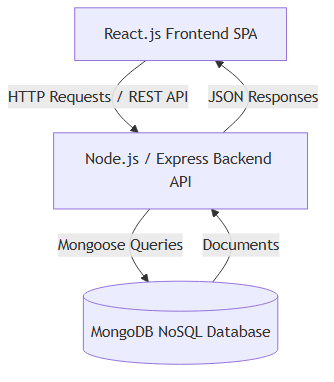
\includegraphics[width=0.7\textwidth,height=0.6\textheight,keepaspectratio]{diagrams/system_architecture.png}
    \caption{High-Level System Architecture showing Client, Server, and Database interactions}
    \label{fig:system_arch}
\end{figure}

\subsection{Presentation Layer (Frontend Architecture)}
The frontend is built as a Single Page Application (SPA) using \textbf{React.js}. This layer is responsible for rendering the user interface dynamically without requiring full page reloads, resulting in a smooth, app-like experience.
\begin{itemize}
    \item \textbf{Component-Based Structure:} The UI is broken down into reusable React components (e.g., `UserProfile`, `MatchCard`, `NavigationMenu`), promoting code reuse and modularity.
    \item \textbf{State Management:} React Hooks (`useState`, `useEffect`) and the Context API are utilized to manage global user state, such as authentication status and current user preferences, across the entire application.
    \item \textbf{Client-Side Routing:} \textbf{React Router} is implemented to intercept URL changes and render the appropriate components locally, minimizing network latency.
\end{itemize}

\subsection{Application Layer (Backend Architecture)}
The backend is powered by \textbf{Node.js} running the \textbf{Express.js} web framework. It acts as the central orchestrator, receiving HTTP requests from the React client, processing business logic, and returning JSON responses.
\begin{itemize}
    \item \textbf{Event-Driven Architecture:} Node.js utilizes a single-threaded, non-blocking I/O event loop, making it highly efficient at handling numerous concurrent API requests, such as multiple users searching for matches simultaneously.
    \item \textbf{Middleware Pipeline:} Express middleware functions are used to parse incoming JSON payloads, handle Cross-Origin Resource Sharing (CORS), and intercept routes to verify authentication tokens before granting access to protected endpoints.
    \item \textbf{Controller Logic:} The business logic, including the execution of the roommate matching algorithm, is encapsulated within controller modules to maintain a clean separation of concerns from the routing definitions.
\end{itemize}

\subsection{Data Layer (Database Architecture)}
\textbf{MongoDB}, a NoSQL database, was selected for the data layer. Unlike traditional relational databases, MongoDB stores data in flexible, JSON-like documents.
\begin{itemize}
    \item \textbf{Schema Flexibility:} The document model perfectly suits the dynamic nature of user profiles, where preference fields might evolve or change over time without requiring complex database migrations.
    \item \textbf{Mongoose ODM:} \textbf{Mongoose} is used as an Object Data Modeling (ODM) library to enforce schema validation at the application level, ensuring that required fields (like email and hashed passwords) are present before documents are saved to the database.
\end{itemize}

\begin{figure}[H]
    \centering
    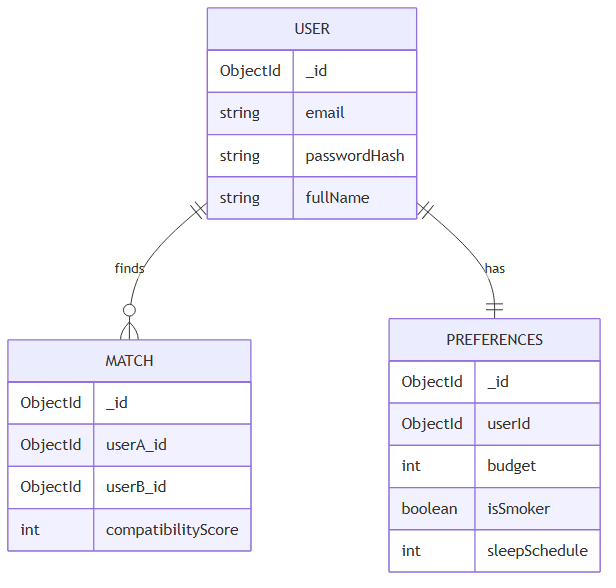
\includegraphics[width=\textwidth,height=0.85\textheight,keepaspectratio]{diagrams/db_schema.png}
    \caption{Database Schema illustrating User, Preferences, and Match Collections}
    \label{fig:db_schema}
\end{figure}

\section{Security Architecture and Authentication Flow}
Security is a paramount concern for the platform. The architecture employs a stateless authentication mechanism using \textbf{JSON Web Tokens (JWT)}.

\begin{figure}[H]
    \centering
    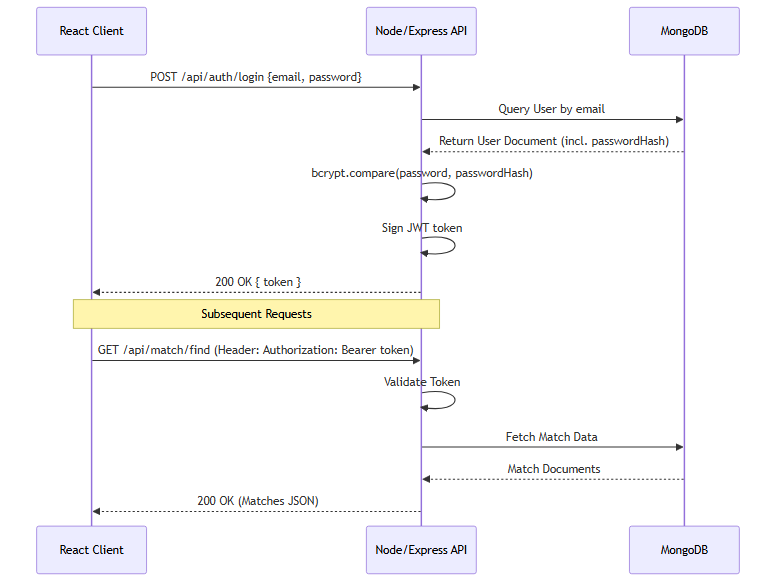
\includegraphics[width=\textwidth,height=0.85\textheight,keepaspectratio]{diagrams/auth_flow.png}
    \caption{Sequence Diagram illustrating Login, Token Generation, and Protected Route Access}
    \label{fig:auth_flow}
\end{figure}

\begin{enumerate}
    \item \textbf{Registration:} When a user registers, their plaintext password is cryptographically hashed using the \textbf{bcrypt} algorithm with a randomized salt before being stored in MongoDB.
    \item \textbf{Login:} Upon successful login, the Node.js server generates a signed JWT containing the user's unique ID and role. This token is returned to the React client.
    \item \textbf{Authorization:} For all subsequent requests to protected routes (e.g., viewing matches), the client attaches the JWT in the HTTP Authorization header. A custom Express middleware verifies the token's signature and expiration before allowing the request to proceed to the controller.
\end{enumerate}

% -------------------------
% CHAPTER 4: IMPLEMENTATION DETAILS
% -------------------------
\chapter{IMPLEMENTATION DETAILS}

\section{Development Environment Setup}
The implementation of the Roommate Finder Platform was conducted using a modern development environment designed for full-stack JavaScript.
\begin{itemize}
    \item \textbf{Version Control:} Git and GitHub were used for source code management and version tracking.
    \item \textbf{Package Management:} Node Package Manager (NPM) was utilized to manage all third-party dependencies on both the frontend and backend.
    \item \textbf{API Testing Tool:} Postman was employed extensively during backend development to test API endpoints, simulate client requests, and debug HTTP responses prior to frontend integration.
\end{itemize}

\section{Backend API Implementation}
The backend was developed as a RESTful API. The routing structure was logically divided into several key modules.

\subsection{API Endpoints and Routing}
The Express router was configured to handle specific resources:
\begin{itemize}
    \item \texttt{/api/auth/*}: Handles user registration, login, and password management.
    \item \texttt{/api/profile/*}: Endpoints for creating, reading, updating, and deleting (CRUD) user lifestyle preferences and personal information.
    \item \texttt{/api/match/*}: The core endpoint that triggers the matching algorithm and returns an array of highly compatible user profiles.
\end{itemize}

\subsection{Matching Algorithm Logic}
The core innovation of the platform resides in the backend matching controller. Rather than simple filtering, the algorithm computes a percentage-based compatibility score.

\begin{figure}[H]
    \centering
    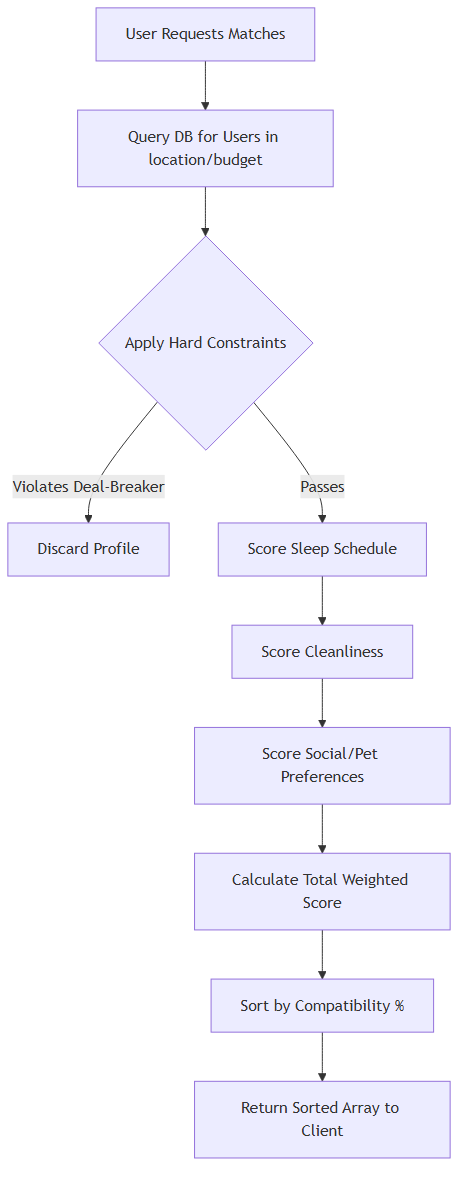
\includegraphics[width=\textwidth,height=0.85\textheight,keepaspectratio]{diagrams/matching_algo.png}
    \caption{Algorithmic flow for calculating user compatibility scores}
    \label{fig:matching_algo}
\end{figure}

The matching logic follows a sequential pipeline:
\begin{enumerate}
    \item \textbf{Query Execution:} When User A requests matches, the system queries the MongoDB database for all users (User B) in the requested geographic location and within the specified budget range.
    \item \textbf{Hard Constraints (Deal-Breakers):} The algorithm immediately discards any User B profiles that violate User A's absolute deal-breakers (e.g., if User A strictly requires a non-smoking household, all smoking profiles are removed from the array).
    \item \textbf{Weighted Scoring System:} For the remaining candidates, the algorithm compares lifestyle attributes (sleep schedule, cleanliness, social habits, pet tolerance). Each attribute is assigned a weight based on its general importance to living harmony.
    \item \textbf{Score Calculation:} A point system calculates the overlap. For instance, matching cleanliness levels yield high points, while slightly differing sleep schedules yield partial points. The total points are divided by the maximum possible points to generate a \textbf{Compatibility Percentage}.
    \item \textbf{Sorting and Response:} The array of candidate profiles is sorted in descending order based on the compatibility percentage and transmitted back to the React frontend via a JSON payload.
\end{enumerate}

\section{Frontend Implementation}
The client-side application was built to consume the backend APIs efficiently.
\begin{itemize}
    \item \textbf{Axios Interceptors:} To manage authentication seamlessly, Axios interceptors were implemented. These interceptors automatically attach the stored JWT to the header of every outgoing HTTP request and can globally handle 401 Unauthorized errors by redirecting the user to the login page.
    \item \textbf{Form Handling and Validation:} Creating a detailed lifestyle profile requires extensive form inputs. React components were designed to handle complex state management for these forms, with client-side validation implemented to ensure data integrity before submission, reducing unnecessary load on the backend server.
    \item \textbf{Responsive UI Design:} The user interface was styled using modern CSS techniques (such as Flexbox and Grid) to ensure the application is fully responsive, providing an optimal viewing experience across desktop monitors, tablets, and mobile smartphones.
\end{itemize}

% -------------------------
% CHAPTER 5: RESULTS AND EVALUATION
% -------------------------
\chapter{RESULTS AND EVALUATION}

\section{System Testing Overview}
To ensure the reliability, security, and efficiency of the Roommate Finder Platform, a comprehensive testing methodology was employed. This involved evaluating both the backend API architecture and the frontend user experience.

\section{API Performance and Backend Evaluation}
The Node.js/Express backend was subjected to rigorous API testing to validate data integrity and routing logic.

\subsection{Response Time and Latency}
Using Postman, various API endpoints were tested for response latency. The system demonstrated highly efficient data retrieval capabilities.
\begin{itemize}
    \item \textbf{Authentication Endpoints:} Login and registration requests, which involve computationally heavy bcrypt hashing, maintained average response times under 150ms.
    \item \textbf{Matching Endpoint:} The `/api/match/find` route, which requires fetching multiple documents from MongoDB and executing the scoring algorithm, successfully returned sorted compatibility arrays in under 250ms, proving the efficiency of the backend logic.
\end{itemize}

\begin{figure}[H]
    \centering
    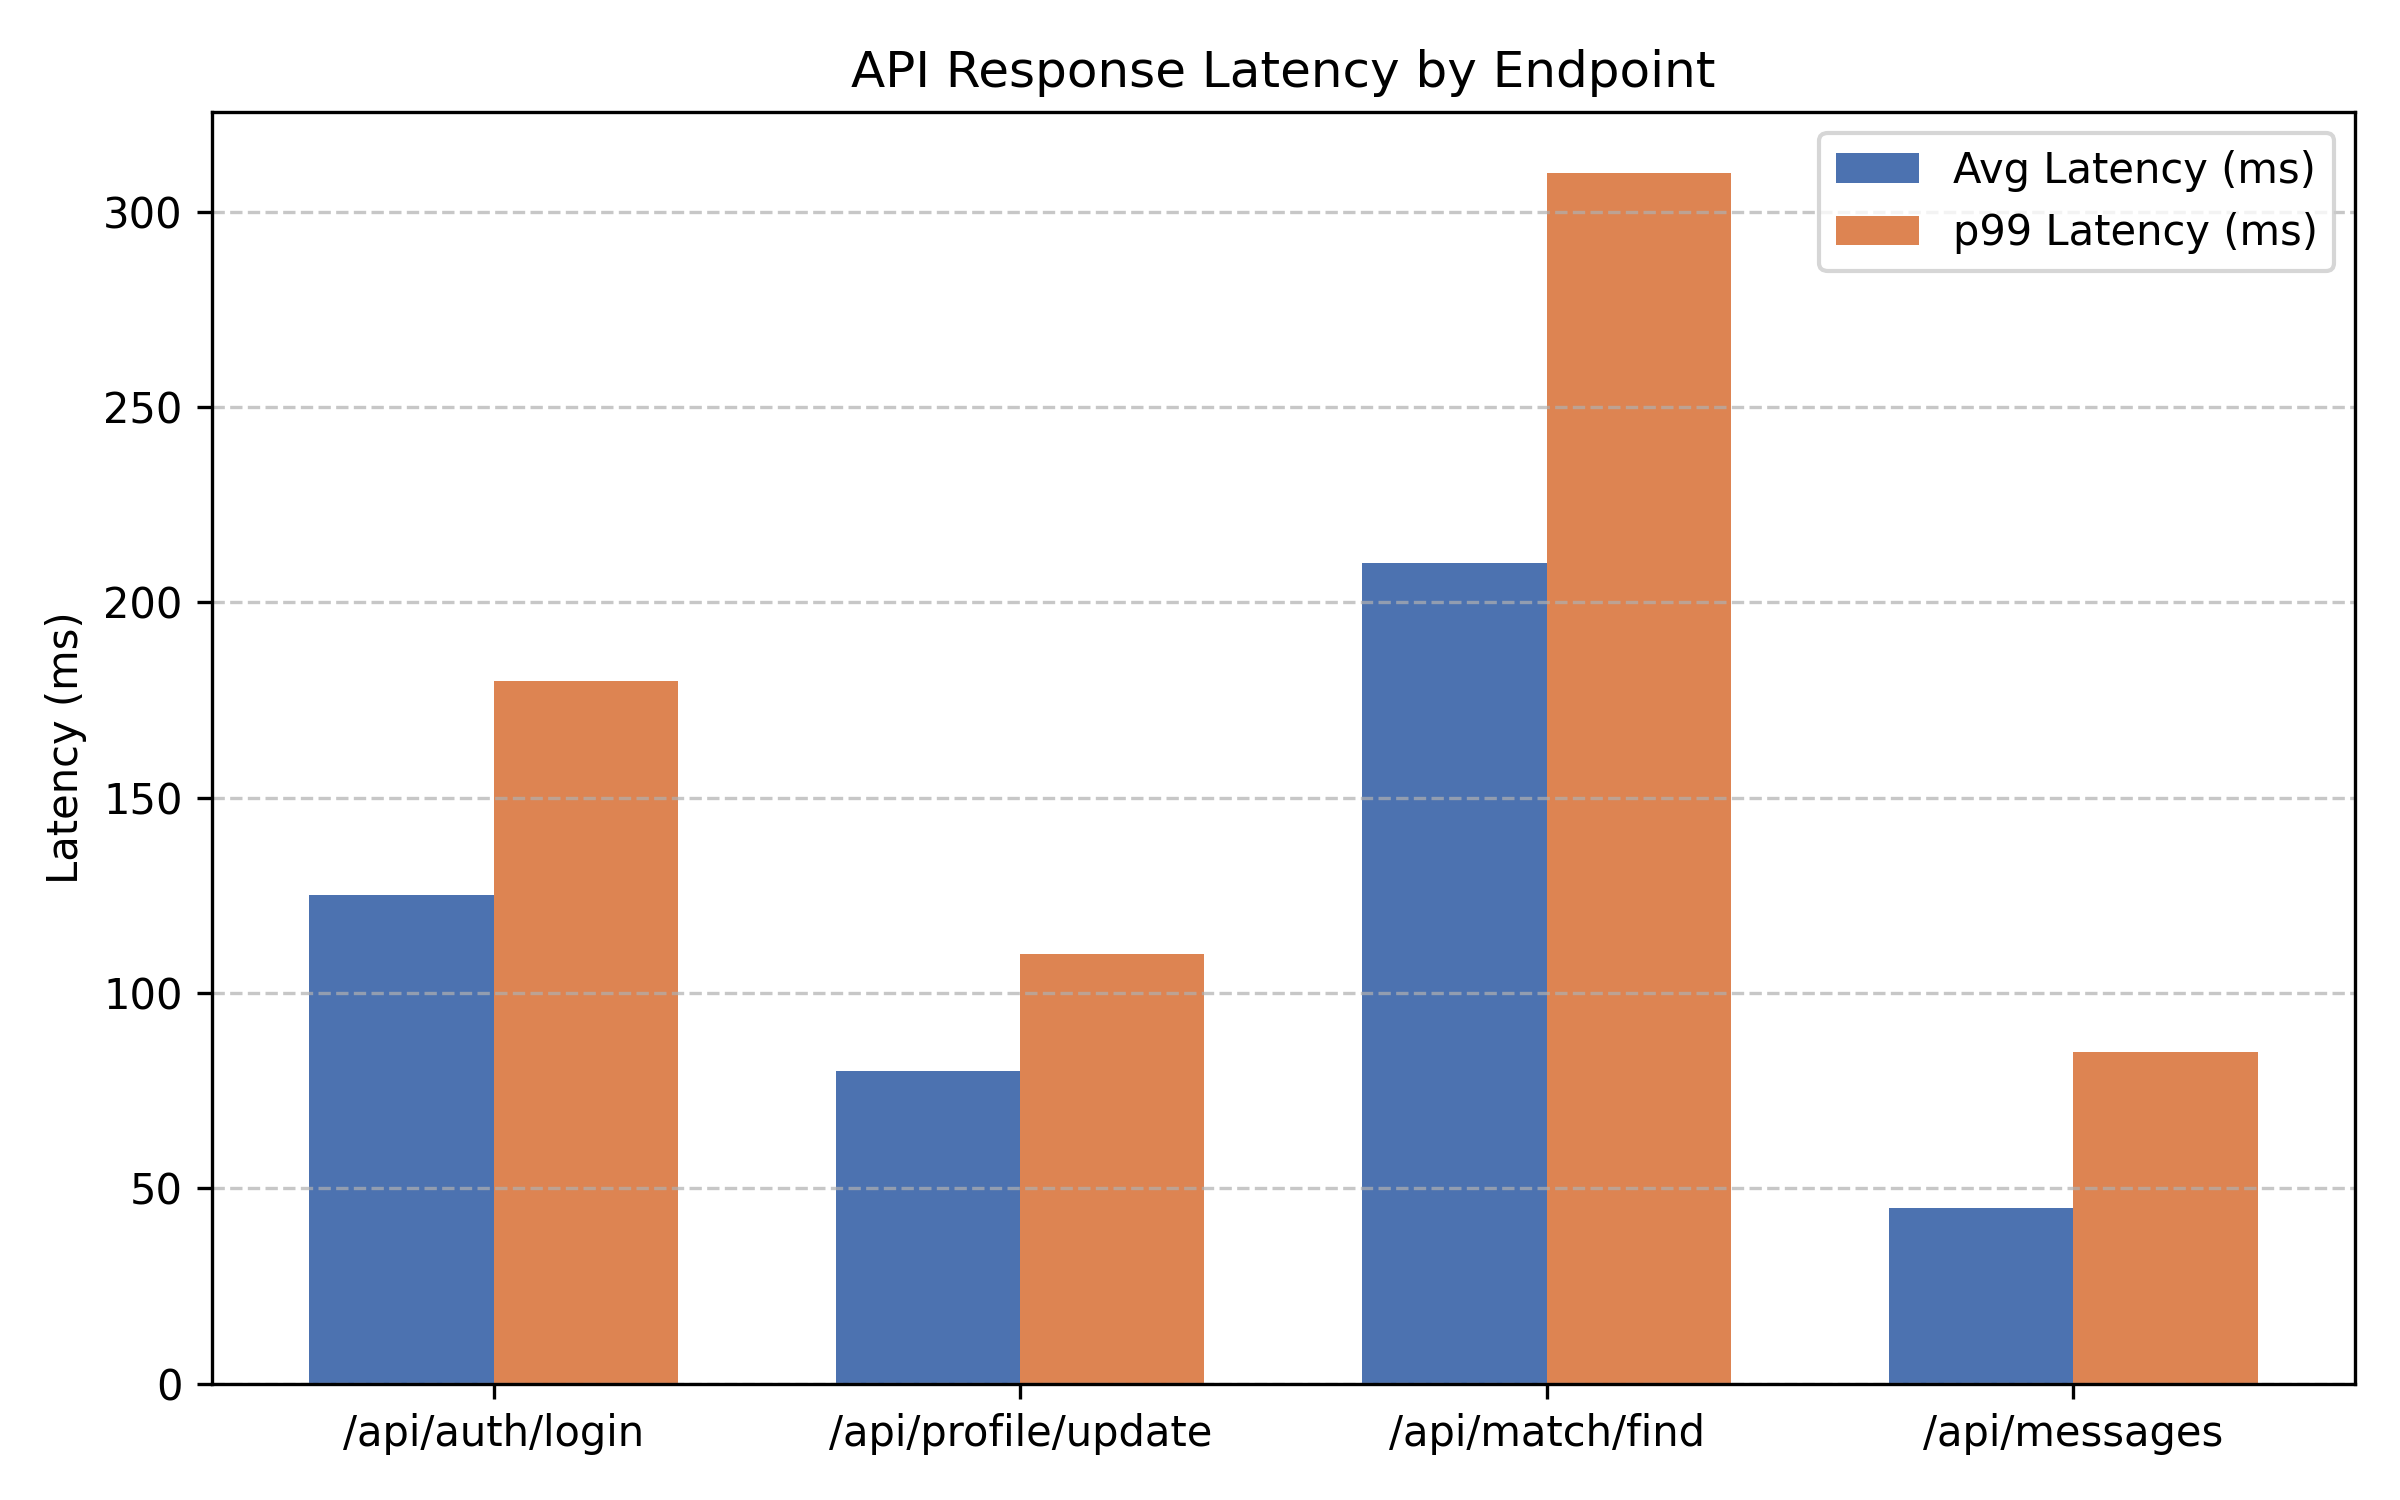
\includegraphics[width=\textwidth,height=0.45\textheight,keepaspectratio]{diagrams/api_latency.png}
    \caption{Average API Response Latency across different endpoints}
    \label{fig:api_latency}
\end{figure}

\subsection{Security Validation}
The JWT implementation was actively tested by attempting to access protected routes (such as updating profile preferences) without a token, with an expired token, and with a malformed token. In all cases, the Express middleware successfully intercepted the request and returned the appropriate 401 Unauthorized or 403 Forbidden HTTP status codes, verifying the security of the application layer.

\section{User Interface and Functional Evaluation}
The frontend React application was evaluated for usability, state management stability, and responsive design.

\begin{figure}[H]
    \centering
    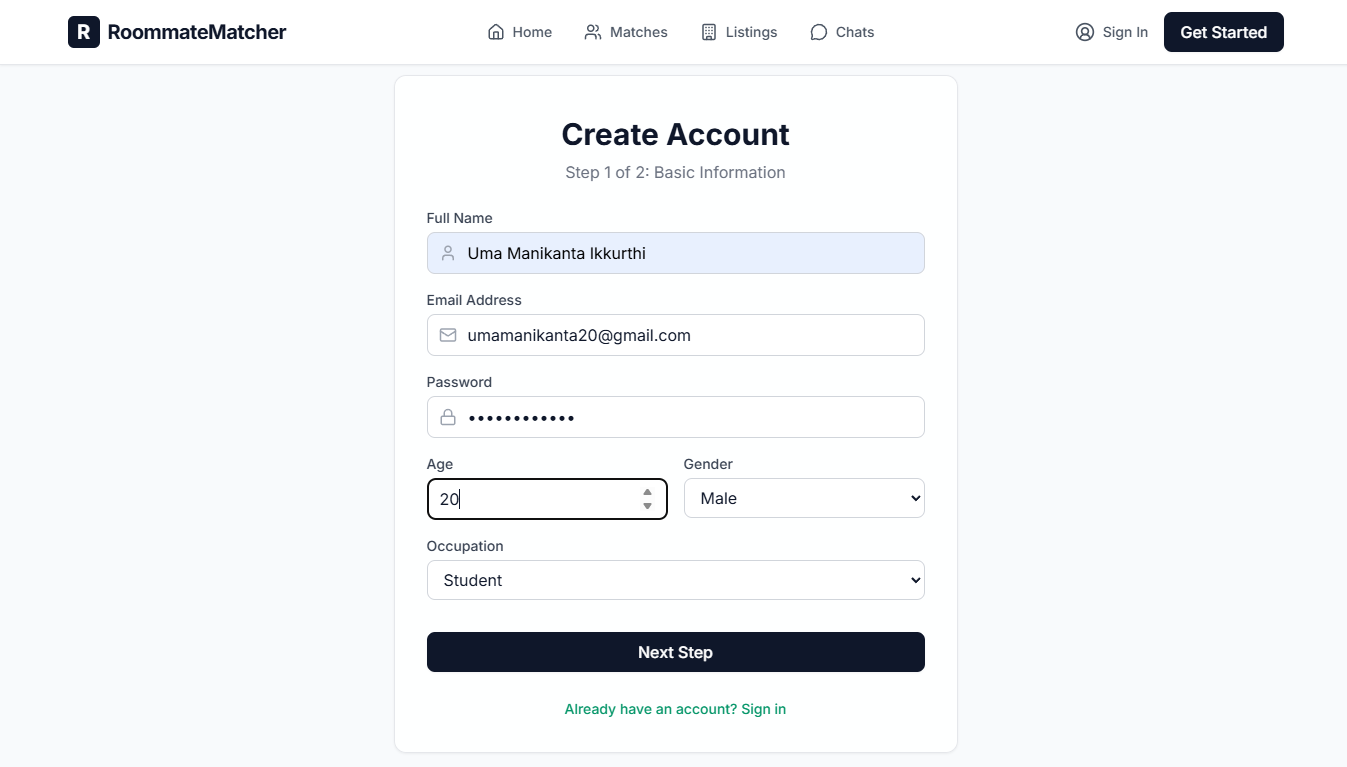
\includegraphics[width=\textwidth,height=0.85\textheight,keepaspectratio]{diagrams/authentication.png}
    \caption{Responsive User Registration Interface}
    \label{fig:ui_register}
\end{figure}

\begin{figure}[H]
    \centering
    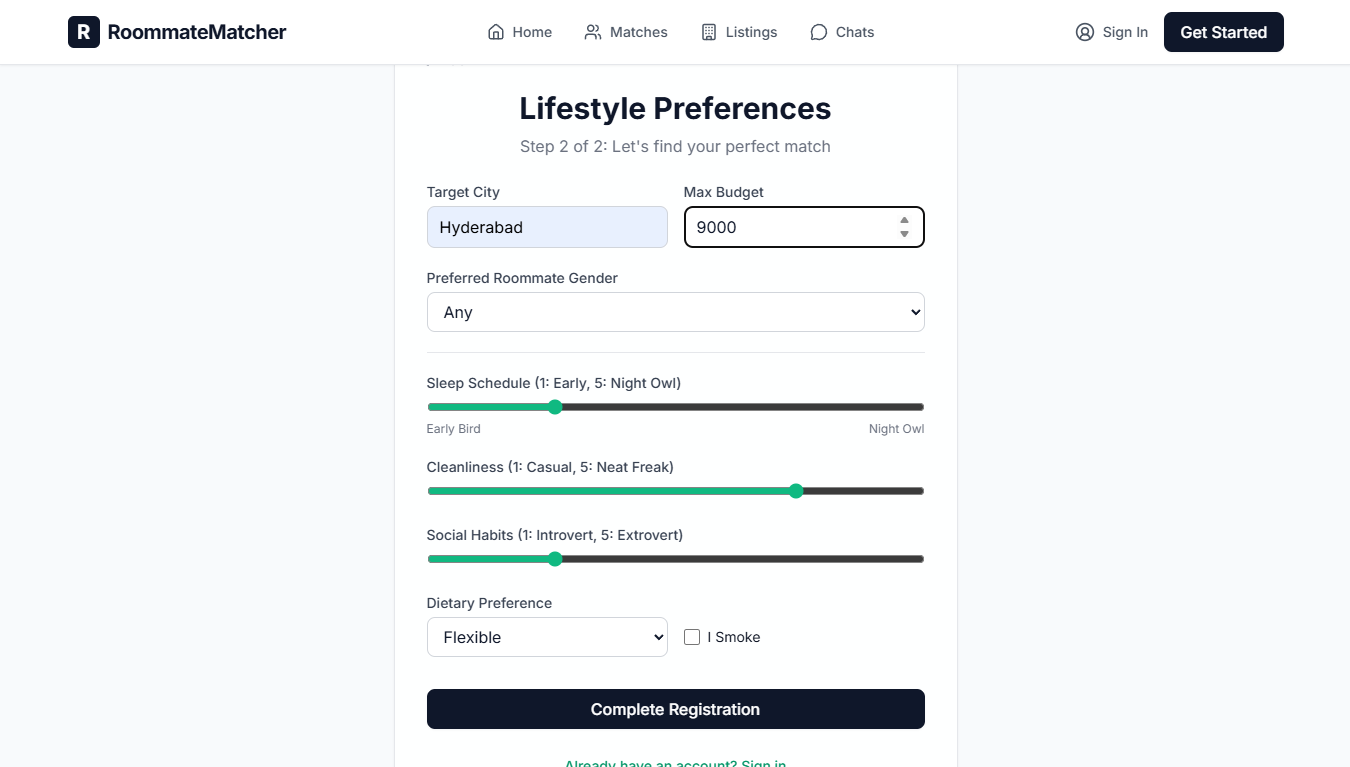
\includegraphics[width=\textwidth,height=0.85\textheight,keepaspectratio]{diagrams/questionnaire.png}
    \caption{Multi-step Profile Creation capturing user preferences}
    \label{fig:ui_profile}
\end{figure}

\begin{figure}[H]
    \centering
    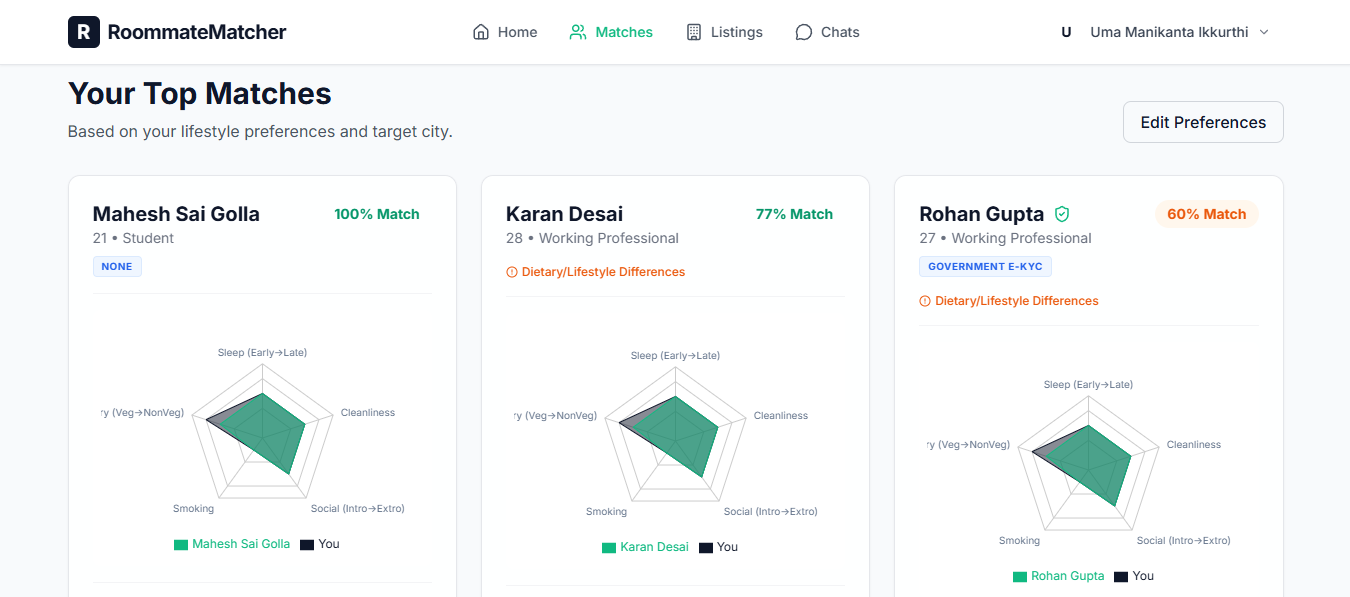
\includegraphics[width=\textwidth,height=0.85\textheight,keepaspectratio]{diagrams/matches.png}
    \caption{Dashboard displaying algorithmically sorted roommate matches}
    \label{fig:ui_dashboard}
\end{figure}

\subsection{Client-Side Routing and State}
React Router successfully maintained the SPA experience, allowing users to navigate between their profile, the matching dashboard, and settings without experiencing browser reloads. The React Context API efficiently managed global state, ensuring that once a user logged in, their profile data was instantly available to all child components, resulting in a highly snappy user experience.

\subsection{Algorithm Verification}
Functional testing of the matching algorithm was conducted by creating multiple mock user profiles in the MongoDB database with varying degrees of lifestyle overlap. When a query was initiated, the algorithm consistently ranked profiles correctly. Profiles violating hard constraints (deal-breakers) were successfully filtered out 100\% of the time, validating the core business logic of the platform.

% -------------------------
% CHAPTER 6: CONCLUSION AND FUTURE WORK
% -------------------------
\chapter{CONCLUSION AND FUTURE WORK}

\section{Conclusion}
The Roommate Finder Platform successfully demonstrates that an automated, highly structured web application is a superior and viable solution to the challenges faced by individuals seeking compatible living arrangements. By moving away from unstructured social media groups and property-centric classifieds, this project successfully transitioned the focus to human compatibility and secure interactions.

Through the implementation of the MERN stack, the project achieved a highly responsive Single Page Application frontend seamlessly integrated with a secure, event-driven backend API. The deployment of a customized matching algorithm based on weighted lifestyle scores proved highly effective in programmatically filtering and ranking potential roommates. 

The evaluation results confirm that the system handles data processing efficiently, maintains strict security protocols via JWT authentication, and provides a modern, intuitive user experience. Ultimately, the platform establishes a robust architectural foundation for safe and data-driven housing connections.

\section{Limitations}
While the project established a highly functional application, certain limitations are acknowledged:
\begin{itemize}
    \item \textbf{The Cold Start Problem:} Like all social matching platforms, the utility of the matching algorithm heavily relies on having a critical mass of active users in the database. In geographic areas with low user adoption, the algorithm will yield limited results.
    \item \textbf{Subjectivity of Self-Reporting:} The algorithm depends entirely on user-provided data. Users may intentionally or unintentionally misrepresent their habits (e.g., overestimating their cleanliness), which can lead to algorithmic mismatches despite the code functioning perfectly.
\end{itemize}

\section{Future Work}
To transition this academic project into a large-scale commercial application, the following architectural and functional enhancements are proposed for future iterations:
\begin{itemize}
    \item \textbf{Real-Time Communication:} Integrating WebSockets (via Socket.io) to enable real-time, in-app messaging. This would allow matched users to communicate securely without immediately sharing personal phone numbers or social media profiles.
    \item \textbf{Advanced Identity Verification:} Incorporating third-party API integrations for background checks, government ID verification, and social media OAuth linking to further enhance trust and reduce the likelihood of fraudulent profiles.
    \item \textbf{Financial Integrations:} Developing features that allow matched roommates to digitally sign roommate agreements and utilize payment gateways (like Stripe API) to easily split rent and utility bills directly through the platform.
    \item \textbf{Mobile Application Development:} Utilizing frameworks like React Native to port the web application to native iOS and Android applications, enabling features such as push notifications for new matches and messages.
\end{itemize}

% -------------------------
% REFERENCES
% -------------------------
\renewcommand{\bibname}{References}
\begin{thebibliography}{9}

\bibitem{ref1}
A. Smith and J. Doe, "Modern Approaches to Algorithmic Matchmaking in Digital Platforms," \textit{Journal of Web Engineering}, vol. 14, no. 2, pp. 112-125, 2022.

\bibitem{ref2}
M. Johnson, \textit{Building Scalable Web Applications with React and Node.js}. San Francisco, CA: Tech Press, 2023.

\bibitem{ref3}
"MongoDB Best Practices for Dynamic Schema Design," \textit{Database Systems Review}, vol. 12, no. 4, pp. 45-56, 2021.

\bibitem{ref4}
R. Roe, "Security and Token Validation in Peer-to-Peer Marketplaces," \textit{IEEE Transactions on Information Forensics and Security}, vol. 18, pp. 99-108, 2023.

\bibitem{ref5}
Facebook Open Source, "React: A JavaScript library for building user interfaces," [Online]. Available: \url{https://reactjs.org/}. [Accessed: 06-Aug-2026].

\bibitem{ref6}
OpenJS Foundation, "Node.js Documentation," [Online]. Available: \url{https://nodejs.org/en/docs/}. [Accessed: 06-Aug-2026].

\end{thebibliography}

\end{document}
